% !Mode:: "TeX:UTF-8"
\chapter{人工数据集上的\cosync运行结果}
以下是本次在人工数据集上进行的部分结果,每一幅图的左边为原始数据矩阵,每一个色块的轮廓代表一个联合簇;右边为\cosync完成联合后的结果。
\vspace{4mm}
\pic[!htb]{单个联合簇}{width=140mm}{ap1}
\pic[!htb]{双联合簇,对角分布}{width=140mm}{ap2}
\newpage
\begin{figure}
\centering
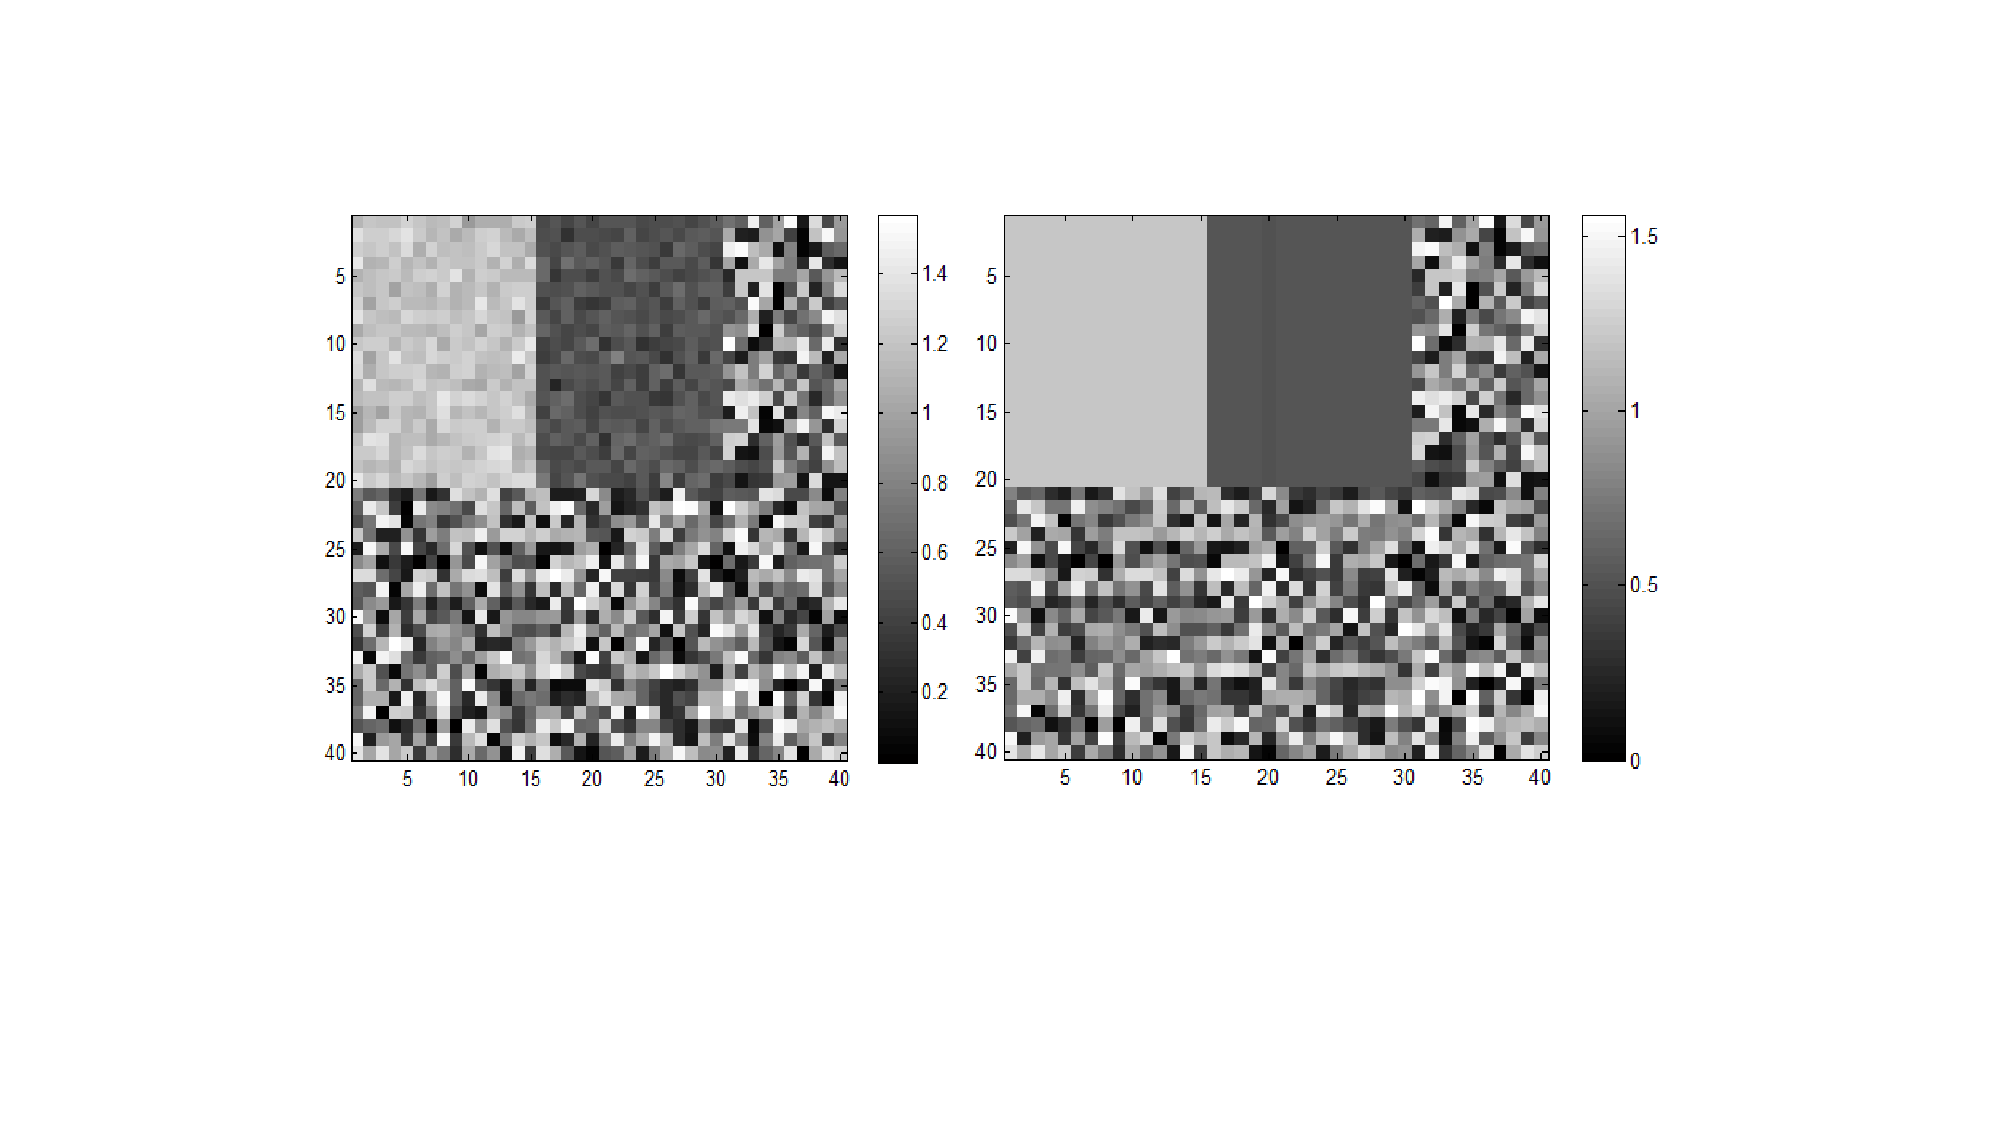
\includegraphics[width=140mm]{ap3}
\caption {双联合簇,并排分布}
\label{fig:idea}
\end{figure}

\begin{figure}
\centering
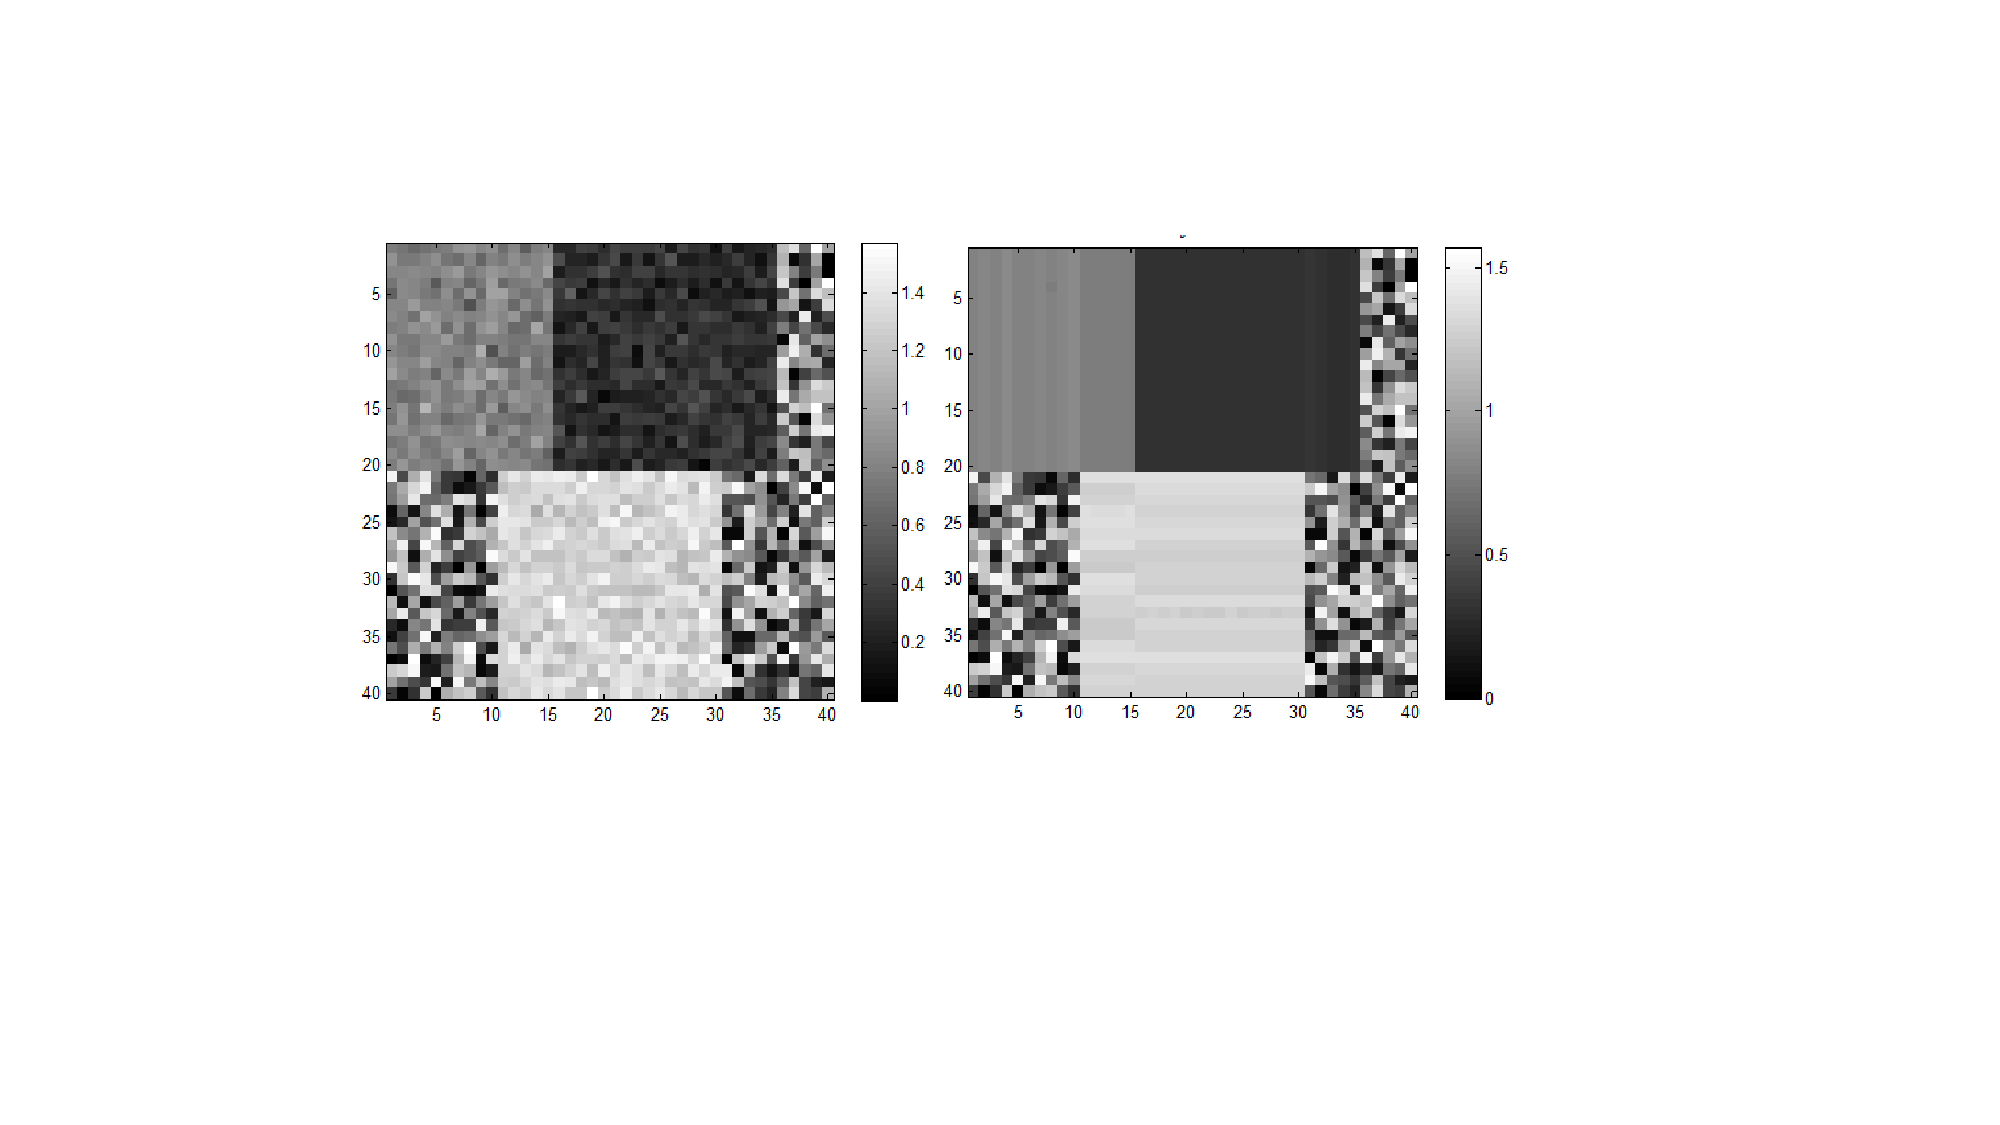
\includegraphics[width=140mm]{ap4}
\caption {三联合簇,不规则分布}
\label{fig:idea}
\end{figure}

\begin{figure}
\centering
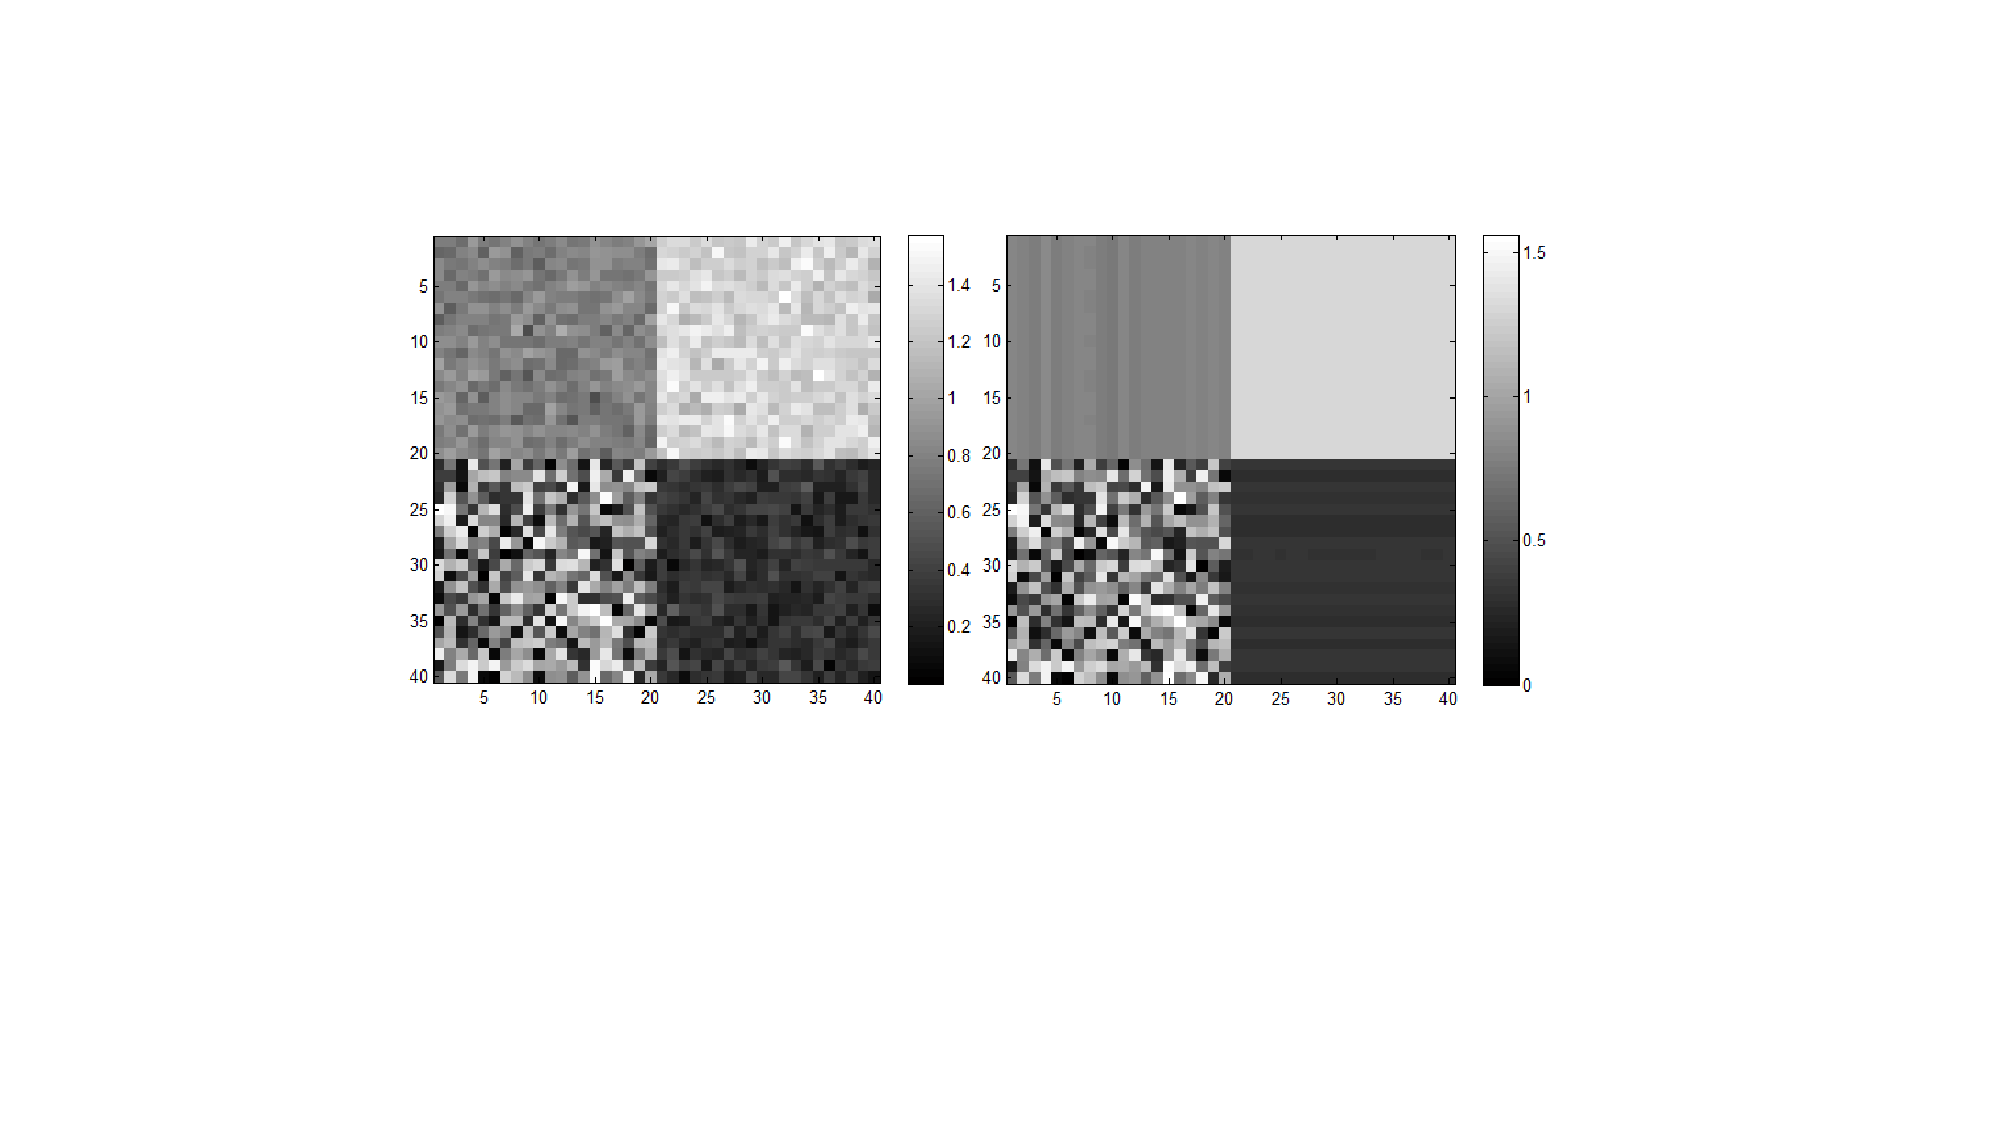
\includegraphics[width=140mm]{ap5}
\caption {三联合簇,规则分布}
\label{fig:idea}
\end{figure}

% \vspace{-8mm}
% \pic[!htb]{双联合簇,并排分布}{width=140mm}{ap3}
% \vspace{-4mm}
% \pic[!htb]{三联合簇,不规则分布}{width=140mm}{ap4}
% \vspace{-4mm}
% \pic[!hb]{三联合簇,规则分布}{width=140mm}{ap5}
% \vspace{-4mm}
